\begin{frame}{Что такое Git}
      \begin{columns}
            \begin{column}{0.6\textwidth}
                  \begin{itemize}
                        \item
                              Git -- распределенная система управления версиями.
                        \item
                              Git хранит наборы изменений между разными версиями проекта, называемые фиксациями
                        \item
                              Каждый коммит указывает на предшествующий ему (или предшествующие), таким образом образуется дерево коммитов
                    \end{itemize}
            \end{column}
            \begin{column}{0.4\textwidth}
                  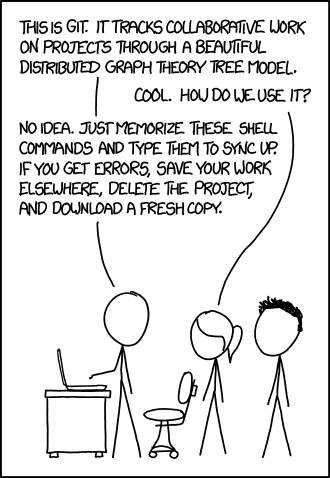
\includegraphics[width=\textwidth,height=0.8\textheight,keepaspectratio]{images/memes/git.png}
            \end{column}
      \end{columns}    
\end{frame}